\documentclass[11pt,a4paper]{article}
\usepackage[utf8]{inputenc}
\usepackage[margin=1in]{geometry}
\usepackage{amsmath,amssymb}
\usepackage{graphicx}
\usepackage{booktabs}
\usepackage{hyperref}
\usepackage{xcolor}
\usepackage{microtype}
\usepackage{fancyhdr}
\usepackage{titlesec}
\usepackage{enumitem}

\raggedbottom
\emergencystretch=3em

\definecolor{emeraldgreen}{HTML}{10B981}
\definecolor{darkslate}{HTML}{0F172A}
\definecolor{deepcyan}{HTML}{0EA5E9}

\hypersetup{
    colorlinks=true,
    linkcolor=emeraldgreen,
    filecolor=deepcyan,      
    urlcolor=deepcyan,
    pdftitle={Overleaf Studio - System Architecture & Technical Specifications},
    pdfpagemode=FullScreen,
}

\pagestyle{fancy}
\fancyhf{}
\rhead{\textcolor{gray}{System Architecture Specification}}
\lhead{\textcolor{emeraldgreen}{\textbf{Overleaf Studio LaTeX IDE}}}
\cfoot{\thepage}

\title{
    \vspace{-1.5cm}
    \textbf{\Huge Overleaf Studio}\\
    \vspace{0.3cm}
    \textbf{\Large System Architecture \& Technical Specification Document}\\
    \vspace{0.2cm}
    \large Open-Source Real-Time LaTeX to PDF Web IDE \& AI Copilot Engine
}

\author{
    \textbf{Core Engineering Team}\\
    \textit{Antigravity Advanced Agentic Coding}
}
\date{\today}

\begin{document}

\maketitle
\thispagestyle{empty}

\begin{abstract}
This document outlines the comprehensive technical architecture, design patterns, framework allocations, and execution workflows of \textbf{Overleaf Studio}—a high-performance, open-source LaTeX to PDF Web IDE. The system unifies client-side code editing via Monaco Editor, multi-stage compilation using the standalone Tectonic LaTeX engine, automated syntax healing and box badness resolution, and an integrated AI LaTeX Copilot Agent into a portable, production-ready containerized platform.
\end{abstract}

\vspace{0.5cm}
\hrule
\vspace{0.5cm}

\tableofcontents
\newpage

\section{System Architecture Overview}

Overleaf Studio is structured as a decoupled 5-tier architecture that guarantees sub-second compilation, fault-tolerant rendering, multi-file workspace persistence, and intelligent AI-guided code corrections.

\begin{figure}[htbp]
\centering
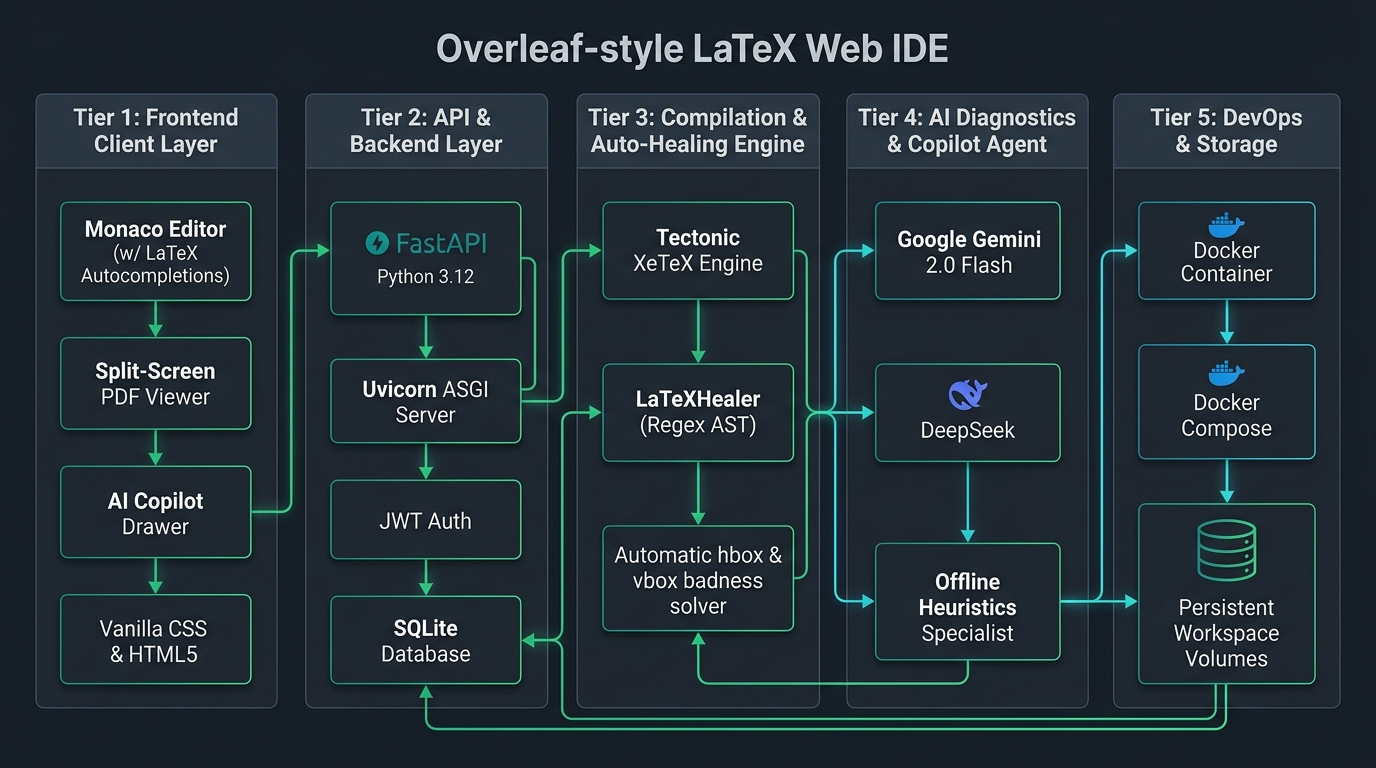
\includegraphics[width=0.95\linewidth]{system_architecture.png}
\caption{High-Level 5-Tier System Architecture Diagram of Overleaf Studio.}
\label{fig:arch}
\end{figure}

\section{Technical Tier Breakdown}

\subsection{Tier 1: Frontend Client Presentation Layer}
\begin{itemize}[leftmargin=1.5em]
    \item \textbf{Monaco Editor (VS Code Web Engine)}: Serves as the primary LaTeX code editing surface, customized with the \textit{Dark Emerald} Overleaf design system.
    \item \textbf{Intelligent Autocomplete Provider (\texttt{latex-completions.js})}: Injects over 100+ LaTeX mathematical commands, environments (\texttt{align}, \texttt{bmatrix}, \texttt{figure}), Greek letters, and dynamic scanners for \texttt{\textbackslash ref\{\dots\}} labels and \texttt{\textbackslash cite\{\dots\}} BibTeX entries.
    \item \textbf{Split-Screen PDF Controller (\texttt{pdf-viewer.js})}: Embedded zero-latency PDF rendering viewport with hardware-accelerated zoom controls and auto-compile synchronizer.
    \item \textbf{AI Copilot Slide-Over Drawer (\texttt{ai-copilot.js})}: Glassmorphic copilot interface with quick-action chips, prompt input, markdown explanation renderer, and 1-click \textit{Apply to Editor \& Compile} action.
    \item \textbf{Vanilla CSS3 Design System}: Zero-dependency, performant responsive layouts with CSS grid, flexbox, and CSS variables.
\end{itemize}

\subsection{Tier 2: Backend Application \& API Layer}
\begin{itemize}[leftmargin=1.5em]
    \item \textbf{FastAPI (Python 3.12)}: High-throughput asynchronous REST API framework handling project CRUD, multi-file I/O, compilation requests, AI streaming, and asset uploads.
    \item \textbf{Uvicorn ASGI Server}: Production-grade async server managing concurrent connections and non-blocking sub-process workers.
    \item \textbf{Security \& Authentication (\texttt{auth.py})}: Salted password hashing via \texttt{bcrypt} (12 rounds) and stateless JWT sessions with \texttt{HS256} signatures.
    \item \textbf{SQLite Database (\texttt{database.py})}: Lightweight embedded relational database enforcing foreign key cascades across \texttt{users}, \texttt{projects}, and \texttt{project\_files}.
    \item \textbf{Server-Side Rendering (Jinja2)}: Fast initial page loads for auth screens, dashboards, and editor workspaces.
\end{itemize}

\subsection{Tier 3: Compilation \& Auto-Healing Engine}
\begin{itemize}[leftmargin=1.5em]
    \item \textbf{Tectonic LaTeX Engine (XeTeX)}: Standalone, multi-package LaTeX compiler capable of on-the-fly package resolution without requiring a 4GB TeXLive install.
    \item \textbf{Intelligent Healer (\texttt{LaTeXHealer})}: Fault-tolerant multi-stage compiler pipeline that intercepts compilation failures and applies regex-based AST repairs:
    \begin{enumerate}
        \item Literal comment operator escaping: \texttt{\textbackslash text\{Accuracy (\%)\}} $\rightarrow$ \texttt{\textbackslash text\{Accuracy (\textbackslash\%)\}}.
        \item Math paragraph break cleaner: Converts illegal blank lines in math mode to comments (\texttt{\%}).
        \item Unclosed command balancing: Auto-closes unclosed \texttt{\textbackslash text\{\dots\}}, \texttt{\textbackslash textbf\{\dots\}}, and bracket pairs.
        \item Unclosed environment resolution: Injects missing \texttt{\textbackslash end\{itemize\}}, \texttt{\textbackslash end\{align\}}, \texttt{\textbackslash end\{document\}}.
        \item Dynamic package discovery: Auto-imports \texttt{amsmath}, \texttt{amssymb}, \texttt{graphicx}, \texttt{booktabs}, \texttt{hyperref}, \texttt{xcolor}.
    \end{enumerate}
    \item \textbf{Automated \texttt{\textbackslash hbox} \& \texttt{\textbackslash vbox} Solver}: Automatically injects \texttt{\textbackslash raggedbottom} (solving \texttt{Underfull \textbackslash vbox (badness 10000)}), \texttt{\textbackslash usepackage\{microtype\}} (solving \texttt{Overfull \textbackslash hbox}), and \texttt{\textbackslash emergencystretch=3em}.
\end{itemize}

\subsection{Tier 4: AI Diagnostics \& Copilot Agent}
\begin{itemize}[leftmargin=1.5em]
    \item \textbf{Multi-Model Orchestration (\texttt{ai\_agent.py})}:
    \begin{itemize}
        \item \textbf{Google Gemini 2.0 Flash}: Ultra-fast 1M token context reasoning via REST API and Google GenAI SDK.
        \item \textbf{Free Public LLMs}: Zero-config free online model fallback (DeepSeek-V3 / Llama-3.3).
        \item \textbf{Offline Heuristics Specialist}: Deterministic rule-based LaTeX expert engine running locally without internet access or API keys.
    \end{itemize}
    \item \textbf{Structured JSON Output}: Produces standardized explanations, change summaries, and full drop-in replacement source code.
\end{itemize}

\subsection{Tier 5: DevOps, Containerization \& Persistent Storage}
\begin{itemize}[leftmargin=1.5em]
    \item \textbf{Docker Multi-Stage Container}: Minimal Debian-based image bundling native Linux Tectonic, font libraries, and Python 3.12.
    \item \textbf{Docker Compose}: Single-command orchestration mapping persistent volumes (\texttt{./data:/app/data}) and port \texttt{8000:8000}.
    \item \textbf{Workspace Sandboxing}: Strictly isolated user directory paths (\texttt{data/workspaces/\{user\_id\}/\{project\_id\}/}) preventing cross-tenant access.
\end{itemize}

\section{Data Flow \& Execution Pipeline}

\begin{enumerate}
    \item \textbf{Editing Phase}: The user types LaTeX source in Monaco Editor. The client-side autocomplete engine suggests commands, labels, and citations.
    \item \textbf{Debounced Sync}: After 1200ms of idle typing (or on \texttt{Ctrl+Enter}), the active file content is saved via \texttt{POST /api/projects/\{id\}/files}.
    \item \textbf{Compilation Trigger}: \texttt{POST /api/projects/\{id\}/compile} invokes the multi-stage compiler pipeline.
    \item \textbf{Stage 1 (Direct)}: Tectonic compiles the document. If return code is 0, the output PDF is served immediately.
    \item \textbf{Stage 2 (Auto-Heal)}: If errors occur, \texttt{LaTeXHealer} repairs syntax bugs in memory, writes \texttt{\_build\_main.tex}, recompiles, and copies the resulting PDF to \texttt{main.pdf}.
    \item \textbf{Live Rendering}: The PDF viewer displays the fresh PDF; compiler notices and auto-fixes are populated in the diagnostics drawer.
    \item \textbf{AI Consultation}: The user can open the AI Copilot to ask questions, fix box warnings, or auto-apply refined code directly into Monaco.
\end{enumerate}

\section{Security Architecture}

\begin{table}[htbp]
\centering
\begin{tabular}{@{}lll@{}}
\toprule
\textbf{Security Domain} & \textbf{Threat Vector} & \textbf{Mitigation Strategy} \\
\midrule
Authentication & Brute-force / Credential theft & Salted \texttt{bcrypt} (12 rounds) + HttpOnly JWT cookies \\
Database & SQL Injection (SQLi) & 100\% Parameterized queries via SQLite driver \\
File System & Directory Path Traversal & \texttt{os.path.basename} sanitization on all file operations \\
Multi-Tenancy & Cross-User Data Access & User-ID verification middleware on all endpoints \\
Execution Sandbox & Command Injection & Safe sub-process argument lists (no \texttt{shell=True}) \\
\bottomrule
\end{tabular}
\caption{Security Controls \& Threat Mitigation Matrix.}
\label{tab:security}
\end{table}

\section{Conclusion}

Overleaf Studio delivers a robust, zero-dependency alternative to complex cloud LaTeX platforms. By combining asynchronous Python backend architecture, local standalone compiler binaries, automated fault-tolerant healing heuristics, and cutting-edge AI assistance, it establishes a reliable foundation for scientific and technical document authoring.

\end{document}
